\begin{tikzpicture}

% Signal
\node[
    %label=north:{\Large{Application of the Short-Time Fourier Transform}},
    label=east:{\Huge{\textbf{\dots}}},
    label={[label distance=0.6cm]west:{\large{Signal}}}
] (signal) at (0, 0) {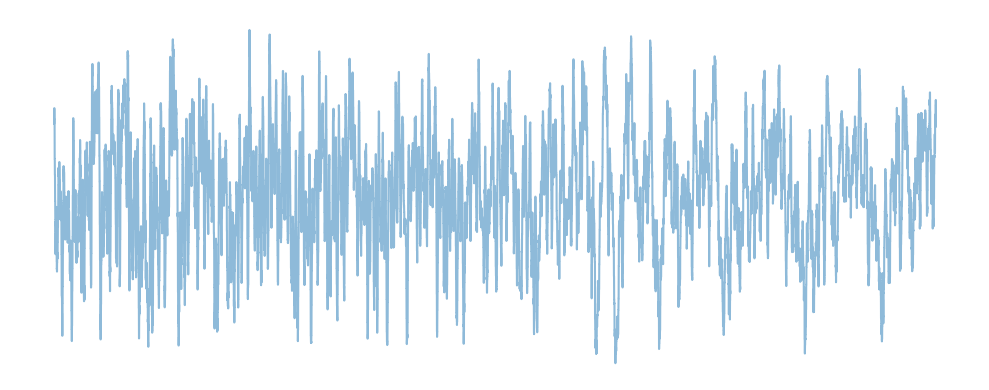
\includegraphics[scale=0.42]{figures/stftfull}};


% Window
\node[
    label=east:{\Huge{\textbf{\dots}}},
    label=west:{\large{Windows}},
    below=0.3cm of signal,
    xshift=-0.2cm
] (windows) {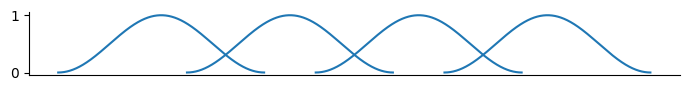
\includegraphics[scale=0.62,trim={0 0.25cm 0 0.2cm},clip]{figures/stftwindows}};

% Window Arrows
\draw[<->] ($(windows.north west) + (1.05, 0)$) -- ($(windows.north) - (1.25, 0)$) 
node[above, midway] (windowlabel) {\footnotesize{Window Length}};
\draw[<->] ($(windows.south west) + (1.05, 0)$) -- ($(windows.south) - (2.5, 0)$) 
node[below, midway] {\footnotesize{Hop Length}};


% Windows
\node[
    below=2cm of windowlabel
] (window0) {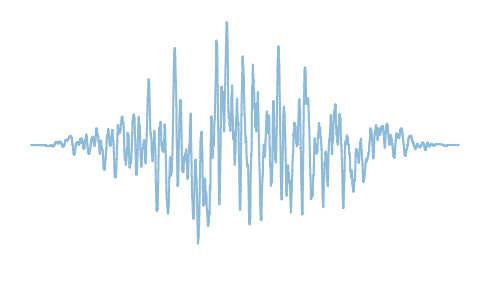
\includegraphics[scale=0.35]{figures/stftwindow0}};
\node[
    below right=-1.75cm and -1.8cm of window0,
    label={[label distance=3cm]west:{\parbox{2.5cm}{\centering \large{Windowed \\ Signal}}}}
] (window1) {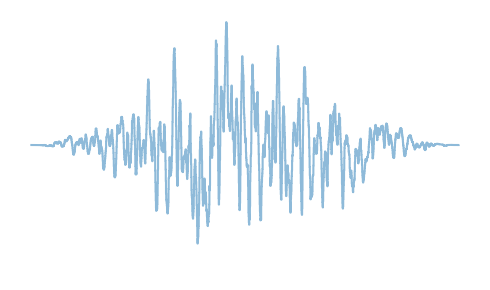
\includegraphics[scale=0.35]{figures/stftwindow1}};
\node[
    below right=-1.75cm and -1.8cm of window1,
    label={[rotate=-45]south east:{\Huge{\textbf{\dots}}}}
] (window2) {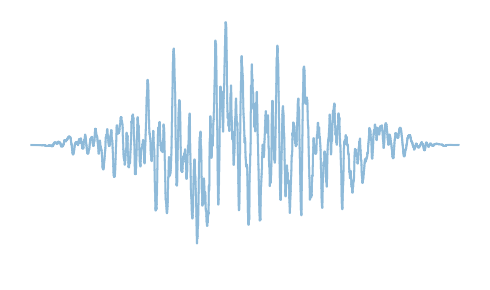
\includegraphics[scale=0.35]{figures/stftwindow2}};


% FFTs
\coordinate (fftarrow) at ($(window1.west |- window2.north) + (0, -1)$);
\draw[->, thick] (fftarrow) -- ($(fftarrow) + (0, -2.45)$) node[left, midway] {\large{FFT}};

\node[
    label=east:{\Huge{\textbf{\dots}}},
    below=1.25cm of window2,
    label={[label distance=-0.25cm]north:{\footnotesize{FFT Output 3}}}
] (fft2) {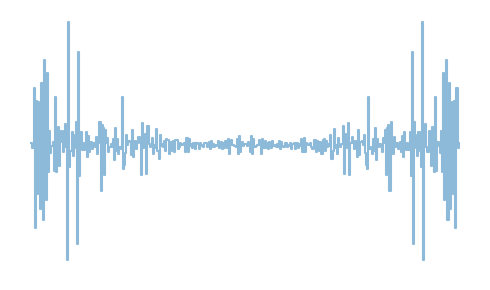
\includegraphics[scale=0.2]{figures/stft2}};
\node[
    left=0.15cm of fft2,
    label={[label distance=-0.25cm]north:{\footnotesize{FFT Output 2}}}
] (fft1) {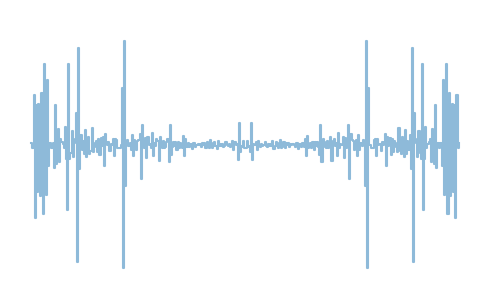
\includegraphics[scale=0.2]{figures/stft1}};
\node[
    left=0.15cm of fft1,
    label={[label distance=-0.25cm]north:{\footnotesize{FFT Output 1}}},
    label={[label distance=0.82cm]west:{\parbox{2.5cm}{\centering \large{Frequency \\ Spectra}}}}
] (fft0) {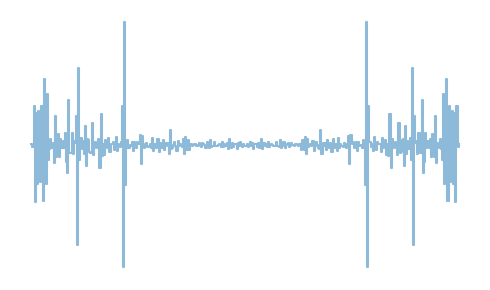
\includegraphics[scale=0.2]{figures/stft0}};

\end{tikzpicture}